\documentclass[11pt,letterpaper]{article}

%====================================================================
% 1. MATEMÁTICA Y FUENTES
%====================================================================

% Compilador: XeLaTeX
\usepackage{fontspec}
\usepackage{amsmath}
\usepackage{mathtools}
\usepackage{amsthm}
\usepackage{amssymb}
\usepackage{unicode-math}

%====================================================================
% 2. IDIOMA
%====================================================================

\usepackage{polyglossia}
\setmainlanguage{spanish}

\usepackage{csquotes}
\usepackage{etoolbox}

%====================================================================
% 3. DISEÑO Y FORMATO GENERAL
%====================================================================

\usepackage[margin=1in]{geometry}

\usepackage{microtype}
\usepackage{setspace}
\usepackage{enumitem}
\usepackage{ragged2e}

% Interlineado
\setstretch{1.1}

% Configuración de párrafos
\setlength{\parindent}{1.2em}
\setlength{\parskip}{0pt}
\setlength{\emergencystretch}{2em}

% Configuración de listas
\setlist{
    itemsep=2pt,
    topsep=4pt
}

%====================================================================
% 4. TABLAS
%====================================================================

\usepackage[table]{xcolor}

\usepackage{booktabs}
\usepackage{tabularx}
\usepackage{longtable}
\usepackage{array}

%====================================================================
% 5. FIGURAS Y ELEMENTOS GRÁFICOS
%====================================================================

\usepackage{graphicx}
\usepackage{float}
\usepackage{caption}
\usepackage{pdflscape}

% Configuración de títulos de tablas y figuras
\captionsetup{
    font=small,
    labelfont=bf,
    labelsep=period,
    skip=6pt
}

%====================================================================
% 6. CÓDIGO Y LISTADOS
%====================================================================

\usepackage{listings}

\lstset{
    language=Python,
    basicstyle=\ttfamily\small,
    frame=lines,
    keywordstyle=\bfseries,
    commentstyle=\itshape\color{gray},
    showstringspaces=false,
    columns=fullflexible,
    xleftmargin=1em
}

%====================================================================
% 7. ENCABEZADOS Y PIES DE PÁGINA
%====================================================================

\usepackage{fancyhdr}

\setlength{\headheight}{15pt}

\pagestyle{fancy}
\fancyhf{}

\renewcommand{\headrulewidth}{0pt}

\fancyhead[R]{
    \small\itshape Informe de avance del proyecto
}

\fancyfoot[C]{
    \small\thepage
}

%====================================================================
% 8. BIBLIOGRAFÍA
%====================================================================

% Procesamiento mediante Biber
\usepackage[
    backend=biber,
    style=authoryear,
    sorting=nyt
]{biblatex}

% Archivo de referencias bibliográficas
\addbibresource{references.bib}

%====================================================================
% 9. ENLACES Y REFERENCIAS CRUZADAS
%====================================================================

\usepackage{xurl}

\usepackage[
    colorlinks=true,
    linkcolor=blue!40!black,
    citecolor=blue!40!black,
    urlcolor=blue!40!black,
    pdfusetitle
]{hyperref}

\hypersetup{
    pdftitle={Informe de avance del proyecto},
    pdfauthor={Anthonny Flores Rojas,
               Andrey Gonzalez Bastos,
               Diego Vega}
}

\usepackage[capitalise]{cleveref}

% Nombres utilizados en las referencias cruzadas
\crefname{theorem}{Teorema}{Teoremas}
\crefname{proposition}{Proposición}{Proposiciones}
\crefname{lemma}{Lema}{Lemas}
\crefname{corollary}{Corolario}{Corolarios}
\crefname{definition}{Definición}{Definiciones}
\crefname{example}{Ejemplo}{Ejemplos}
\crefname{conjecture}{Conjetura}{Conjeturas}
\crefname{section}{Sección}{Secciones}
\crefname{table}{Tabla}{Tablas}
\crefname{figure}{Figura}{Figuras}
\crefname{equation}{ecuación}{ecuaciones}

%====================================================================
% 10. TEOREMAS Y ENTORNOS MATEMÁTICOS
%====================================================================

% Numeración de teoremas por sección
\theoremstyle{plain}

\newtheorem{theorem}{Teorema}[section]
\newtheorem{proposition}[theorem]{Proposición}
\newtheorem{lemma}[theorem]{Lema}
\newtheorem{corollary}[theorem]{Corolario}
\newtheorem{conjecture}[theorem]{Conjetura}

\theoremstyle{definition}

\newtheorem{definition}[theorem]{Definición}
\newtheorem{example}[theorem]{Ejemplo}

\theoremstyle{remark}

\newtheorem{remark}[theorem]{Observación}

% Numeración de ecuaciones por sección
\numberwithin{equation}{section}

% Nombre de las demostraciones
\gappto\captionsspanish{%
    \renewcommand{\proofname}{Demostración}
}

%====================================================================
% 11. COMANDOS MATEMÁTICOS
%====================================================================

\newcommand{\R}{\mathbb{R}}
\newcommand{\Z}{\mathbb{Z}}
\newcommand{\E}{\mathbb{E}}

\renewcommand{\P}{\mathbb{P}}

\newcommand{\dd}{\,\mathrm{d}}

\newcommand{\norm}[1]{%
    \lVert #1\rVert
}

\newcommand{\Sh}{\mathcal{S}}

\DeclareMathOperator{\LSE}{LSE}

%====================================================================
% 12. ENTORNOS MATEMÁTICOS EN ESPAÑOL
%====================================================================

\newtheorem{teorema}[theorem]{Teorema}
\newtheorem{proposicion}[theorem]{Proposición}
\newtheorem{lema}[theorem]{Lema}
\newtheorem{corolario}[theorem]{Corolario}
\newtheorem{definicion}[theorem]{Definición}
\newtheorem{ejemplo}[theorem]{Ejemplo}
\newtheorem{observacion}[theorem]{Observación}

%====================================================================
% 13. COMANDOS PARA MONEDAS
%====================================================================

\newcommand{\eur}{\texttt{EUR}\,}
\newcommand{\gbp}{\texttt{GBP}\,}
\newcommand{\czk}{\texttt{CZK}\,}

%====================================================================
% 14. CLASIFICACIÓN DE DATOS
%====================================================================

% Categoría A: datos publicados
\newcommand{\catA}{\textbf{[A]}}

% Categoría B: cálculos propios
\newcommand{\catB}{\textbf{[B]}}

% Categoría C: datos no disponibles o no verificables
\newcommand{\catC}{\textbf{[C]}}

%====================================================================
% 15. COMANDOS AUXILIARES DEL INFORME
%====================================================================

% Resaltar el estado de un elemento
\newcommand{\estado}[1]{\textbf{#1}}

% Entornos de interlineado sencillo
\newcommand{\sw}{\begin{singlespace}}
\newcommand{\ew}{\end{singlespace}}

% Texto provisional
\newcommand{\ph}[1]{%
    \textcolor{red!70!black}{\textit{[#1]}}
}

% Estados para tablas de avance
\newcommand{\done}{%
    \textcolor{green!45!black}{\textbf{Completado}}
}

\newcommand{\wip}{%
    \textcolor{orange!80!black}{\textbf{En curso}}
}

\newcommand{\todo}{%
    \textcolor{red!70!black}{\textbf{Pendiente}}
}

%====================================================================
% 16. DATOS INSTITUCIONALES
%====================================================================

\newcommand{\Universidad}{Universidad de Costa Rica}
\newcommand{\Escuela}{Escuela de Matemáticas}

\newcommand{\Curso}{
    Valoración de instrumentos financieros (CA0308)
}

\newcommand{\Profesor}{
    Daniel Vargas Carrillo
}

%====================================================================
% 17. DATOS DEL DOCUMENTO
%====================================================================

\title{
    \textbf{Nombre del informe}\\[0.4em]
    \large Informe de anteproyecto
}

\author{%
    {Anthonny Flores Rojas}
    \thanks{
        Escuela de Matemáticas,
        Universidad de Costa Rica.
        \texttt{anthonny.flores@ucr.ac.cr}
    }
    \and
    {Andrey Gonzalez Bastos}
    \thanks{
        Escuela de Matemáticas,
        Universidad de Costa Rica.
        \texttt{andrey.gonzalezbastos@ucr.ac.cr}
    }
    \and
    {Diego Vega}
    \thanks{
        Escuela de Matemáticas,
        Universidad de Costa Rica.
        \texttt{diego.vega@ucr.ac.cr}
    }
}

\date{
    Curso: Valoración de instrumentos financieros (CA0308)\\
    Profesor: Daniel Vargas Carrillo\\[0.3em]
    \today
}

\begin{document}
	
	
	\maketitle

	\newpage

	\tableofcontents   % opcional; muchos papers largos lo incluyen

	\newpage
	
% =====================================================================
\section{Introducción}\label{sec:intro}

Giannozzi y Kirilova \parencite{GIANNOZZI2026107700} investigan por qué una cobertura 
con derivados, útil para fijar precios, puede amplificar el riesgo de una empresa en 
un episodio de estrés. Los contratos cotizados se valoran a mercado a diario y exigen
 margen inicial y de variación en efectivo; si el precio del subyacente se mueve contra 
 la posición, la empresa debe aportar liquidez de inmediato aunque la cobertura sea 
 económicamente razonable \parencite[p.~1]{GIANNOZZI2026107700}. Con datos de empresas 
 energéticas europeas durante la crisis de 2022, los autores documentan que la mayoría 
 financia esas llamadas con deuda, que las empresas sin relaciones previas con prestamistas 
 venden activos, y que las llamadas se asocian con mayor riesgo de incumplimiento, 
 mayor costo de la deuda y menores márgenes \parencite[p.~1]{GIANNOZZI2026107700}. 
 Son resultados de la muestra; en este informe se usan como mecanismo explicativo y 
 no se atribuyen a ČEZ.

La selección de ČEZ, a. s., responde a criterios financieros y no a 
la disponibilidad de datos. Primero, la empresa pertenece a la muestra del artículo: 
figura entre las que informan en qué partida del balance registran los depósitos de margen, 
en este caso «cuentas por cobrar comerciales, margen y colaterales» 
\parencite[Apéndice A3, p.~16]{GIANNOZZI2026107700}. Segundo, genera cerca de 58\% 
de la electricidad checa \parencite[p.~11]{cez_fs_2021} y el Estado posee 69,8\% de su 
capital \parencite[p.~10]{cez_interim_q3_2021}. Tercero, vende por adelantado su generación 
y lo cuantifica antes del corte: 79\%, 49\% y 21\% de la generación de 2022, 2023 y 
2024 al 30 de septiembre de 2021 \parencite[p.~27]{cez_interim_q3_2021}. 
Cuarto, su exposición es sobre todo eléctrica (el gas aporta 5,8\% de su generación, 
\parencite{cez_story_2022}), lo que permite aislar un subyacente. 
Quinto, su balance al 30 de septiembre de 2021 se publicó el 9 de noviembre de 2021, 
antes del corte.

El análisis se limita a lo que podía conocerse el \textbf{23 de febrero de 2022}, 
último día hábil anterior al 24 de febrero, cuando se registran los mayores rendimientos 
diarios del gas y la electricidad \parencite[p.~3]{GIANNOZZI2026107700}. Todos los precios, 
volatilidades y probabilidades usan observaciones hasta esa fecha inclusive; los hechos 
posteriores aparecen solo como evidencia retrospectiva (Sección~\ref{sec:sens}). 

\section{Contexto de la empresa y del mercado en la fecha de corte}

\paragraph{Empresa.} ČEZ genera, distribuye y comercializa electricidad y calor, 
además de gas, servicios energéticos y carbón \parencite[p.~10]{cez_interim_q3_2021}. 
Las ventas de electricidad fueron CZK 90.496 millones de unos ingresos operativos de 
CZK 155.955 millones en nueve meses de 2021 (58\% , \parencite[p.~21]{cez_interim_q3_2021}) 
y el segmento de Generación aportó CZK 24.271 millones de un EBITDA consolidado de 
CZK 47.520 millones (51\% , \parencite[pp.~24--25]{cez_interim_q3_2021}). Su estrategia 
combina ventas de electricidad a plazo, compras a plazo de derechos de emisión y 
cobertura del tipo de cambio de ingresos en euros \parencite{cez_q3_2021}. 
El costo ya era visible antes del corte: las preventas redujeron en CZK 4.305 millones 
los ingresos por electricidad de nueve meses porque se liquidaron por debajo del precio 
de mercado \parencite[p.~21]{cez_interim_q3_2021}. La liquidez de referencia al 30 de 
septiembre de 2021 era de CZK 8.023 millones en efectivo \parencite[p.~2]{cez_interim_q3_2021} 
y de CZK 31.400 millones en líneas comprometidas no dispuestas (40.000 menos 8.600 dispuestos; 
cifra de una diapositiva por confirmar \parencite{cez_q3_2021}), frente a una deuda de 
CZK 141.245 millones \parencite[pp.~3, 19, 20]{cez_interim_q3_2021}.

\paragraph{Mercado.} La Tabla~\ref{tab:mercado} resume los indicadores al corte. 
El contrato anual alemán para 2023 cotizaba a EUR 156,43/MWh el 23 de febrero 
de 2022, 82\% más que el 30 de septiembre de 2021 (EUR 85,86) y tres veces el 
nivel de enero de 2021 (EUR 51,25) . En el mercado spot, el promedio diario de 
la subasta Day Ahead pasó de EUR 100,66 (CZ) y 96,84 (DE-LU) en 2021 a EUR 183,22 
y 178,97 en el cuarto trimestre, y a 166,76 y 147,16 entre el 1 de enero y el 
23 de febrero de 2022 . El diferencial medio entre la República Checa y 
Alemania-Luxemburgo fue de EUR 5,85/MWh (5,7\% del precio medio de Alemania-Luxemburgo), 
con correlación de 0,976 entre promedios diarios, y los precios coincidieron en 46,6\% de 
las horas, lo que indica acoplamiento de mercados y un riesgo de base menor que el riesgo 
de nivel.

\sw
\begin{table}[ht]
	\centering
	\footnotesize
		\begin{tabularx}{\textwidth}{@{}>{\RaggedRight}p{3.0cm}>{\RaggedRight}X>{\RaggedRight}p{3.4cm}@{}}
			\toprule
				Indicador & Valor y fecha & Fuente y categoría \\
			\midrule
				Futuro base DE, entrega 2023 & EUR 156,43/MWh (23-feb-2022); 85,86 (30-sep-2021); 51,25 (4-ene-2021) & \textcite{energycharts_futuros_de},  \\
				Futuro base DE, entrega 2024 & EUR 118,88/MWh (23-feb-2022) & ídem,  \\
				Spot Day Ahead CZ / DE-LU & Último día, 23-feb-2022: EUR 136,63 / 130,09 (promedio diario) & \textcite{energycharts_spot2022},  \\
				Gas TTF & EUR 88,85/MWh (23-feb-2022); máximo previo de EUR 182,78 el 21-dic-2021 & \textcite{platts_ttf_2022},  \\
				Derechos de emisión EUA & EUR 94,67/t, contrato más cercano (cierre del 23-feb-2022); EUR 61,66 al 30-sep-2021 & \textcite{gasstrategies_2022}; \parencite[p.~18]{cez_interim_q3_2021},  \\
				EUR/CZK & CZK 24,860 al 31-dic-2021; cotización del 23-feb-2022 pendiente & \parencite[p.~30]{cez_fs_2021},  \\
				Tasas & Repo checa a dos semanas 4,50\% desde el 4-feb-2022 (antes 3,75\%); PRIBOR pendiente & \textcite{cnb_2022},  \\
				Regulación & EMIR: compensación central obligatoria sobre EUR 4.000 millones de nocional bruto en materias primas; sin compensación, valoración diaria y garantías & \parencite[p.~18]{GIANNOZZI2026107700}; norma primaria por verificar, / \\
				Competencia & ČEZ genera cerca de 58\% de la electricidad checa; competidores y cuotas pendientes & \parencite[p.~11]{cez_fs_2021},  \\
			\bottomrule
		\end{tabularx}
	\caption{Estado del mercado en la fecha de corte.}
	\label{tab:mercado}
\end{table}
\ew

El significado financiero de estos niveles es directo. ČEZ vendió 37 TWh de 2022 a 
EUR 54,1/MWh \parencite{cez_q3_2021}, mientras el mercado para años cercanos ya superaba 
EUR 150/MWh: las ventas a plazo estaban muy por debajo del precio de mercado, es decir, 
con pérdida de valoración, antes de que el precio se disparara en febrero. Los derechos 
de emisión se encarecieron 53\% desde septiembre , y ČEZ estima que cada EUR 1/t se 
traslada a la electricidad entre EUR 0,6 y 0,7/MWh \parencite{cez_story_2022}. 
Una repo de 4,50\% encarece además financiar los depósitos de margen. Cuanto mayor 
es el precio, mayor es la pérdida de la posición vendida y, si hay garantías, mayor 
el efectivo que debe aportarse, que es el canal que el artículo identifica.

\section{Subyacente y posición financiera}

El \textbf{subyacente principal} es el precio del futuro anual base de electricidad de 
Alemania con entrega en 2023, cotizado en EEX en EUR/MWh. Se prefiere al spot porque ČEZ 
cubre su producción con ventas a plazo, no con contratos de entrega al día siguiente; 
los precios spot son un indicador complementario y no se mezclan con los de futuros. 
Tampoco se usa el contrato de 2022: su serie termina el 29 de diciembre de 2021, 
de modo que a la fecha de corte no existe un precio anual para ese año, y 
la parte restante de 2022 requeriría precios mensuales o trimestrales que el archivo 
no contiene . El contrato de 2023 es el anual más cercano, con serie continua hasta el 
corte y 49\% de la generación vendida. El de 2024 es secundario. ČEZ informa coberturas 
alemanas para suministros checos de 2021 a 2024 \parencite{cez_q2_2021}, lo que respalda 
el uso del mercado alemán, pero sus documentos no identifican el contrato exacto, la bolsa 
ni la cámara de compensación ; el riesgo de base entre los mercados checo y alemán se acota 
con el diferencial spot de la sección anterior. La serie es homogénea (cada columna es 
un año de entrega fijo, sin empalmes), coincide con valores publicados (EUR 315,00 el 
21 de diciembre de 2021 para 2022 \parencite{platts_2021_dec} y EUR 985,00 el 
26 de agosto de 2022 para 2023 \parencite{eex_2022}) y por eso se interpreta como precios de
 liquidación, aunque el método de extracción requiere verificación (Anexo~D).

La \textbf{posición} se descompone en cuatro capas. La física es larga: 
los ingresos de generación suben con el precio de la electricidad, con entregas 
externas esperadas de 44 a 47 TWh al año \parencite{cez_q3_2021}. La financiera es corta: 
las ventas a plazo fijan un precio y pierden valor cuando el precio sube. 
La económica neta es larga sobre el volumen no vendido, 51\% de 2023 y 79\% de 2024. 
La de liquidez es corta ante alzas: si los contratos se negocian con garantías, 
la pérdida de valoración exige efectivo antes de que se cobre la producción. 
Por eso una cobertura razonable puede generar tensión de liquidez: la compensación 
económica ocurre en la entrega, mientras que la liquidación del margen es diaria. 
El alcance exacto de los derivados sujetos a garantías no consta en los estados revisados; 
solo se sabe que ČEZ registra los depósitos de margen en cuentas por cobrar comerciales 
\parencite[p.~16]{GIANNOZZI2026107700}.

% ===================== 4 =====================

\section{Exposición monetaria y volatilidad}

\paragraph{Exposición.} 
Con 49\% de la generación de 2023 vendida al 30 de septiembre de 2021 y entregas esperadas de
 45,5 TWh (punto medio del rango publicado, supuesto ), el volumen vendido es de 22,3 TWh 
 (21,6 a 23,0 con el rango). Valorado al precio del corte, representa 
 $22{,}3\times156{,}43=\text{EUR }3.488$ millones (CZK 86.700 millones al tipo de cambio 
 de diciembre de 2021); la venta de 2024 (21\%, 9,6 TWh a EUR 118,88) suma EUR 1.136 millones. 
 Esta cifra es el dinero cuyo valor depende del subyacente, no el nocional contable ni 
 el efectivo exigido. El porcentaje vendido es el de septiembre de 2021 y pudo cambiar 
 hasta febrero de 2022; cada diez puntos adicionales sobre 2023 sumarían 4,6 TWh y 
 EUR 712 millones. El precio pactado de 2023 no consta en los documentos; con la media 
 del futuro entre enero y septiembre de 2021 (EUR 61,16/MWh, supuesto) la valoración 
 de la posición corta sería de $-$EUR 2.124 millones, una cifra ilustrativa que 
 probablemente subestima la pérdida si ČEZ vendió antes a precios menores. 
 De los 37 TWh de 2022 quedaban por entregar 31,5 TWh (311 de 365 días, entrega uniforme 
 supuesta), pero sin precio al corte no pueden valorarse.

\paragraph{Volatilidad.} Se calcularon rendimientos logarítmicos diarios del futuro de 
2023 entre el 5 de enero de 2021 y el 23 de febrero de 2022 (295 observaciones) y se 
anualizaron con $\sqrt{252}$ (Tabla~\ref{tab:vol}). La volatilidad se duplica al acortar 
la ventana: de 41\% con todo el historial a 72\% con 60 días, lo que describe un cambio 
de régimen y no un parámetro estable. El máximo rendimiento diario fue 14,0\% (4 de enero 
de 2022). La volatilidad de los precios spot no se calcula en logaritmos porque 
Alemania-Luxemburgo registró 147 horas con precio negativo, y además no equivale a la del 
contrato usado para cubrir.

\sw
\begin{table}[ht]
	\centering
	\footnotesize
		\begin{tabular}{lrrr}
			\toprule
				Estimador (datos hasta 23-feb-2022) & Cal-23 & Cal-24 & Observaciones \\
			\midrule
				60 días & 72,4\% & 42,1\% & 60 \\
				126 días & 57,2\% & 34,4\% & 126 \\
				252 días & 43,7\% & 28,8\% & 252 \\
				Historial completo & 41,2\% & 27,5\% & 295 \\
				EWMA ($\lambda=0{,}94$) & 61,7\% & --- & 295 \\
			\bottomrule
		\end{tabular}
	\caption{Volatilidad anualizada del futuro base alemán (cálculo propio ; Excel, hoja Volatilidad).}
	\label{tab:vol}
\end{table}
\ew

\section{Sensibilidad, probabilidades y conclusiones}\label{sec:sens}

\paragraph{Sensibilidad.} Con $Q_h$ el volumen vendido, $Q_T$ la generación esperada, 
$P_0$ el precio del corte y $s$ la variación, $\Delta V=-Q_hP_0s$ es el cambio de valor de 
la posición corta, $\Delta I=Q_TP_0s$ el de los ingresos físicos y su suma es el efecto neto,
 $(Q_T-Q_h)P_0s$ (Anexo~B). Para 2023, una variación de $\pm10$, $\pm20$ y $\pm30\%$ cambia 
 el valor de la posición vendida en $\mp$EUR 349, 698 y 1.046 millones, mientras que los 
 ingresos físicos varían en $\pm$EUR 712, 1.424 y 2.135 millones; el efecto neto es de 
 $\pm$EUR 363, 726 y 1.089 millones. Si se añade 2024, la variación de la posición vendida 
 llega a $\mp$EUR 1.387 millones (CZK 34.500 millones) con $\pm30\%$. La necesidad de 
 liquidez se acota con $L=\theta\cdot\max(0,-\Delta V)$, donde $\theta$, la fracción de la 
 pérdida aportada en efectivo, no se conoce . Con $\theta=100\%$ y un alza de 30\%, 
 la exigencia es de CZK 34.500 millones, 1,14 veces cubierta por la liquidez de referencia 
 de CZK 39.423 millones; con $\theta=50\%$ sería de CZK 17.200 millones. Dentro de $\pm30\%$ 
 la posición sería manejable respecto de la liquidez de septiembre de 2021, pero el resultado 
 depende de $\theta$, del porcentaje vendido y de que esa liquidez siguiera disponible.

\paragraph{Probabilidades.} Con un modelo lognormal sin tendencia, volatilidad EWMA de 
61,7\% y horizonte de 21 días hábiles (un mes bursátil, supuesto), la probabilidad de un 
alza de al menos 10, 20 y 30\% es de 26,6, 13,3 y 5,9\%; la de una baja, de 30,8, 12,2 y 
2,8\% (Anexo~B). La frecuencia empírica de ventanas de 21 días del propio futuro es 34,2, 
10,5 y 5,1\% para alzas y casi nula para bajas, pero se calcula con ventanas traslapadas 
en una muestra alcista. Son tres conceptos distintos (modelo, historia y escenario) y 
ninguno predice el futuro: el modelo normal subestima las colas y el supuesto de volatilidad 
constante contradice el cambio de régimen de la Tabla~\ref{tab:vol}.

\paragraph{Evidencia posterior, que no estaba disponible al corte.} El mismo futuro llegó a 
EUR 985/MWh el 26 de agosto de 2022 \parencite{eex_2022}, 530\% sobre el precio del corte. 
Aplicado al volumen de 2023, el cambio de valor sería de unos $-$EUR 18.500 millones 
(CZK 459.000 millones ), frente a depósitos de margen que ČEZ informó por más de CZK 195.000 
millones en agosto de 2022 \parencite{cez_pr_2023}, cifra tomada del documento de selección 
y no releída. La rejilla de $\pm30\%$ queda así muy por debajo de la cola que se materializó, 
y la planificación de liquidez debería considerar choques mayores.

\paragraph{Conclusión.} El 23 de febrero de 2022 ČEZ estaba larga en electricidad por su 
generación y corta por unas ventas a plazo que cubrían 49\% de 2023 y 21\% de 2024 con un 
mercado que había triplicado sus precios. Su riesgo central no era económico sino de 
liquidez: las pérdidas de valoración de la posición corta podían exigir efectivo antes del 
cobro de la producción, el mecanismo descrito por Giannozzi y Kirilova. La información 
faltante (precio pactado, fracción con garantías, $\theta$, hedge ratio al corte y precios 
de 2022) se detalla en el Anexo~E.

\section{Gráficos de la serie histórica}

\begin{figure}[H]
\centering
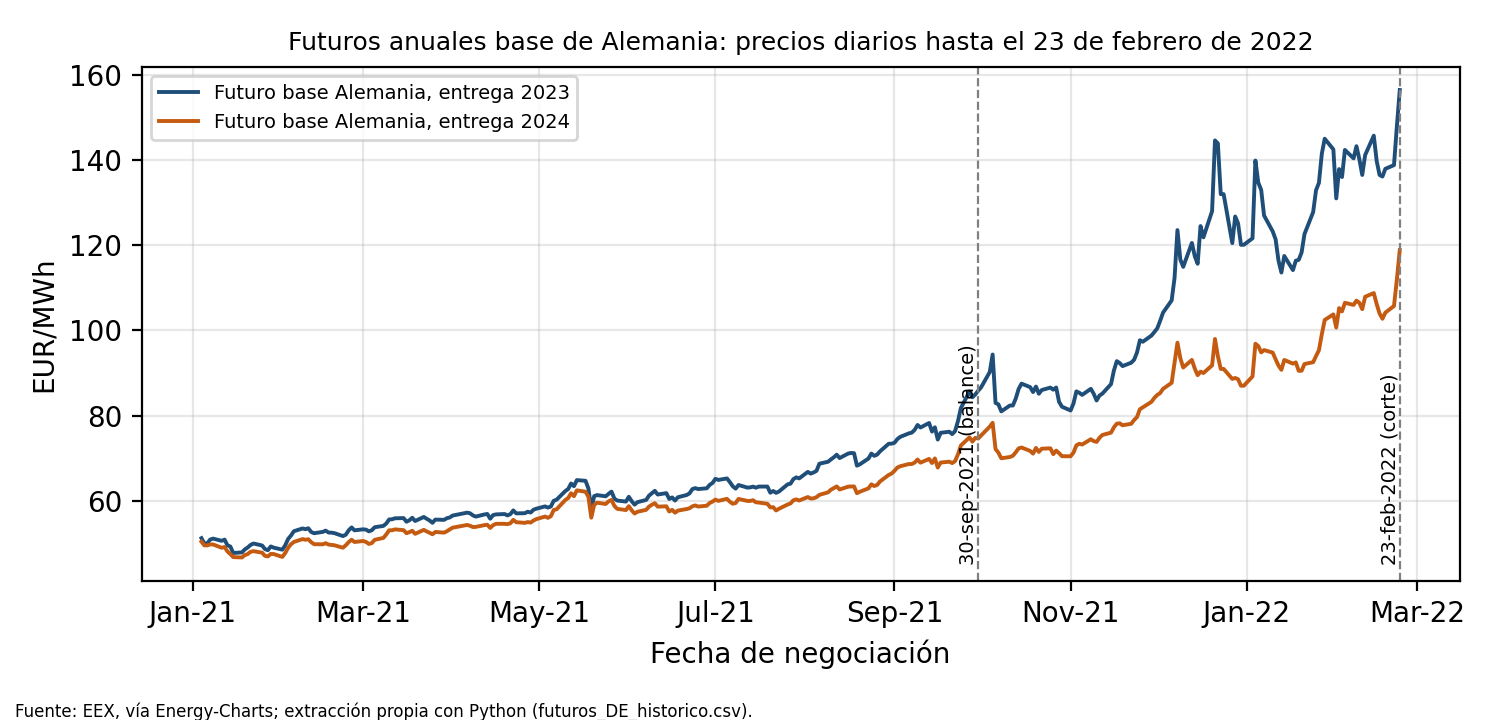
\includegraphics[width=0.95\textwidth]{images/fig_futuros.png}
\caption{Subyacente principal: precios diarios de los futuros anuales base de Alemania para entrega 2023 y 2024, hasta el 23 de febrero de 2022. Fuente: EEX, según Energy-Charts \parencite{energycharts_futuros_de}; extracción propia.}
\end{figure}

\begin{figure}[H]
\centering
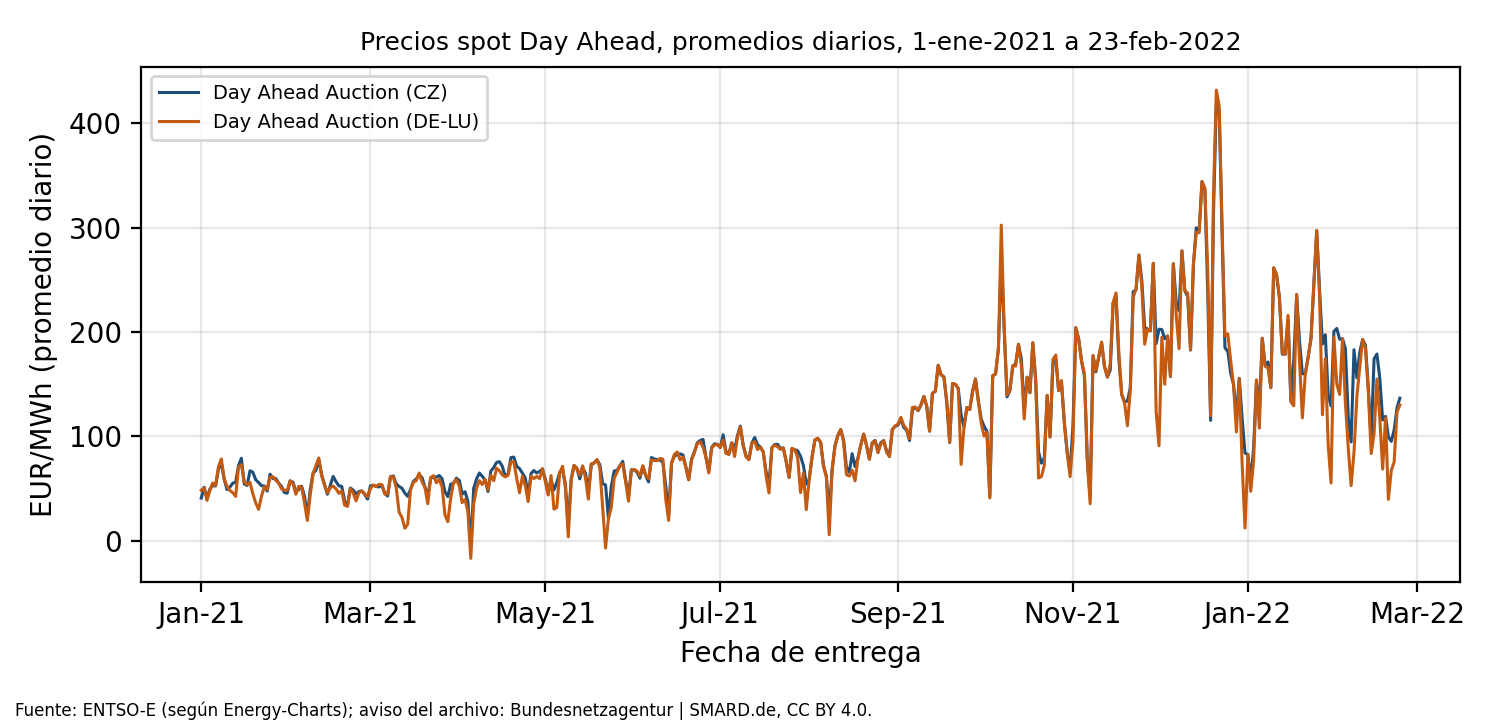
\includegraphics[width=0.95\textwidth]{images/fig_spot.png}
\caption{Contexto spot (no es el subyacente): promedios diarios de la subasta Day Ahead de República Checa y Alemania-Luxemburgo. Fuente: \parencite{energycharts_spot2021,energycharts_spot2022}; los promedios son cálculo propio.}
\end{figure}

\section{Tablas de sensibilidad y probabilidades}

\sw
\begin{table}[H]
\centering
\scriptsize
\setlength{\tabcolsep}{3pt}
\begin{tabular}{rrrrrrrrr}
\toprule
$s$ & $P_0(1+s)$ & $\Delta V$ 2023 & $\Delta I$ 2023 & Neto 2023 & $\Delta V$ 2024 & $\Delta V$ total & $\Delta V$ total & $L$ ($\theta=100\%$) \\
 & EUR/MWh & EUR mill. & EUR mill. & EUR mill. & EUR mill. & EUR mill. & CZK mil mill. & CZK mil mill. \\
\midrule
$-30\%$ & 109,5 & $+1.046$ & $-2.135$ & $-1.089$ & $+341$ & $+1.387$ & $+34,5$ & 0 \\
$-20\%$ & 125,1 & $+698$ & $-1.424$ & $-726$ & $+227$ & $+925$ & $+23,0$ & 0 \\
$-10\%$ & 140,8 & $+349$ & $-712$ & $-363$ & $+114$ & $+462$ & $+11,5$ & 0 \\
$+10\%$ & 172,1 & $-349$ & $+712$ & $+363$ & $-114$ & $-462$ & $-11,5$ & 11,5 \\
$+20\%$ & 187,7 & $-698$ & $+1.424$ & $+726$ & $-227$ & $-925$ & $-23,0$ & 23,0 \\
$+30\%$ & 203,4 & $-1.046$ & $+2.135$ & $+1.089$ & $-341$ & $-1.387$ & $-34,5$ & 34,5 \\
\bottomrule
\end{tabular}
\caption{Sensibilidad. $P_0=156{,}43$, $Q_h=22{,}3$ TWh (2023) y 9,6 TWh (2024), $Q_T=45{,}5$ TWh, CZK 24,860/EUR. Liquidez de referencia: CZK 39,4 mil millones; con $\theta=50\%$, $L$ se reduce a la mitad. Cálculo propio ; supuestos en el Excel.}
\end{table}

\begin{table}[H]
\centering
\footnotesize
\begin{tabular}{lrrrrrr}
\toprule
 & \multicolumn{3}{c}{Alza $\ge x$} & \multicolumn{3}{c}{Baja $\ge x$} \\
\cmidrule(lr){2-4}\cmidrule(lr){5-7}
Estimador de $\sigma$ & 10\% & 20\% & 30\% & 10\% & 20\% & 30\% \\
\midrule
60 días (72,4\%) & 28,8 & 16,4 & 8,7 & 34,5 & 16,8 & 5,5 \\
126 días (57,2\%) & 25,5 & 11,8 & 4,7 & 28,9 & 10,2 & 1,9 \\
252 días (43,7\%) & 20,7 & 6,6 & 1,6 & 22,0 & 4,4 & 0,3 \\
Historial completo (41,2\%) & 19,5 & 5,6 & 1,2 & 20,5 & 3,5 & 0,2 \\
EWMA (61,7\%) & 26,6 & 13,3 & 5,9 & 30,8 & 12,2 & 2,8 \\
\midrule
Frecuencia empírica, 275 ventanas & 34,2 & 10,5 & 5,1 & 0,7 & 0,0 & 0,0 \\
\bottomrule
\end{tabular}
\caption{Probabilidad (\%) de variaciones del futuro Cal-23 en 21 días hábiles: modelo lognormal sin tendencia y frecuencia empírica con ventanas traslapadas.}
\end{table}
\ew

\section{Diagnóstico de los archivos de datos}

\sw
\begin{table}[H]
\centering
\scriptsize
\begin{tabularx}{\textwidth}{@{}>{\RaggedRight}p{3.2cm}>{\RaggedRight}X@{}}
\toprule
Aspecto & Resultado y tratamiento \\
\midrule
Spot 2021 y 2022 & Cada archivo tiene 8.760 registros horarios; la primera fila tras el encabezado contiene unidades y se excluye. Fechas del 1-ene-2021 al 31-dic-2022; marcas con desplazamiento +01:00 y +02:00, de modo que el cambio de horario no genera duplicados ni huecos (días de 23 y 25 horas, uno cada uno). Sin valores faltantes ni duplicados en CZ y DE-LU. Variables: producción (MW) y precios Day Ahead por zona (EUR/MWh). Se retienen 10.056 horas hasta el 23-feb-2022 y se descartan las posteriores. \\
Precios negativos & 33 horas en CZ y 147 en DE-LU: se conservan; impiden rendimientos logarítmicos de promedios diarios. \\
Futuros & 1.494 filas diarias del 4-ene-2021 al 30-oct-2026; una columna por año de entrega (2022 a 2036), en EUR/MWh con dos decimales. Cada columna es un contrato de año fijo con vida limitada (la de 2022 termina el 29-dic-2021, la de 2023 el 28-dic-2022): las celdas vacías corresponden a períodos sin cotización. Sin duplicados; 5 días hábiles ausentes en la serie de 2023; 2 rendimientos nulos. No hay mezcla de vencimientos dentro de una columna, por lo que los rendimientos son comparables; no se calculan entre columnas. \\
Naturaleza de los precios & El archivo no indica si son liquidación o indicativos. Las coincidencias exactas con EUR 985,00 (26-ago-2022) y EUR 315,00 (21-dic-2021) son compatibles con precios de liquidación, sin demostrarlo. \\
\bottomrule
\end{tabularx}
\caption{Control de calidad de los datos.}
\end{table}
\ew

\section{Trazabilidad y método de obtención de los datos}

\textbf{Spot.} Fuente original según Energy-Charts: ENTSO-E; plataforma: Energy-Charts (Fraunhofer ISE); descarga directa de CSV; actualización informada del 27/10/2026 (14:44 y 15:36 CET), aunque los registros son de 2021 y 2022. El aviso del propio archivo atribuye los precios Day Ahead de CZ y DE-LU a Bundesnetzagentur | SMARD.de bajo licencia CC BY 4.0 y reserva el resto de datos para uso privado e interno; por ello el informe cita ambas atribuciones y usa solo esas dos zonas.

\textbf{Futuros.} Fuente original según Energy-Charts: EEX; plataforma de visualización: Energy-Charts. La plataforma no ofrecía descarga directa, por lo que el CSV resulta de un procedimiento propio en Python que accedió a la información de la gráfica. No es un archivo de EEX ni de Energy-Charts. No se adjuntó el código, de modo que no puede afirmarse si extrajo valores numéricos estructurados o reconstruyó valores a partir de coordenadas visuales. La evidencia es favorable a lo primero (valores con dos decimales, fechas de negociación y exactitud de 985,00 y 315,00), pero la verificación queda pendiente: revisar el código y contrastar una muestra de fechas con EEX.

\section{Diagnóstico de cumplimiento y acciones restantes}

\sw
\begin{table}[H]
\centering
\scriptsize
\begin{tabularx}{\textwidth}{@{}>{\RaggedRight}p{3.6cm}>{\RaggedRight}p{1.7cm}>{\RaggedRight}X@{}}
\toprule
Requisito & Estado & Qué falta o condiciona \\
\midrule
1. Empresa, negocio y problema & COMPLETO & Confirmar visualmente cifras de diapositivas. \\
2. Contexto de mercado & PARCIAL & EUR/CZK y PRIBOR al corte; verificar la norma primaria (EMIR) y competidores. \\
3. Subyacente & PARCIAL & Contrato, bolsa y cámara usados por ČEZ (notas IFRS 7/9). \\
4. Posición larga o corta & PARCIAL & Fracción con garantías; porcentaje vendido al corte. \\
5. Exposición monetaria & PARCIAL & Precio pactado de 2023, nocional contable, precios de 2022. \\
6. Volatilidad histórica & PARCIAL & Cálculo hecho; falta verificar el código de extracción. \\
7. Sensibilidad & PARCIAL & $\theta$ y precio pactado. \\
8. Probabilidades & PARCIAL & Hereda la verificación de datos; horizonte es supuesto. \\
9. Gráfico histórico & COMPLETO & Figura 1 del Anexo A. \\
10. Excel auditable & COMPLETO & Generado y recalculado con LibreOffice (16 controles verdaderos); sin revisión independiente. \\
11. Informe de cinco páginas & COMPLETO & Contenido principal en cinco páginas; anexos aparte. \\
12. Presentación de 15 minutos & PENDIENTE & No preparada. \\
\bottomrule
\end{tabularx}
\caption{Matriz de cumplimiento.}
\end{table}
\ew

\textbf{Pendientes por prioridad.} 
\begin{enumerate}
    \item Indispensable: estados consolidados de ČEZ de 2021, notas 18 y 19 (págs.~81--94), para el contrato, el nocional y las garantías; informe de resultados del tercer trimestre de 2021 para el precio pactado de 2023 y el porcentaje vendido, a confirmar visualmente. 
    \item Indispensable: código Python de extracción y contraste con EEX. 
    \item Indispensable: preparar la presentación. 
    \item Complementario: cotización EUR/CZK de la ČNB y PRIBOR del 23-feb-2022; precios mensuales de EEX para el resto de 2022; reglamento delegado de EMIR en EUR-Lex; depósitos de margen de 2022 releídos en los comunicados de ČEZ; sustituir réplicas de documentos por enlaces oficiales.
\end{enumerate}

\clearpage
  \printbibliography[title={Referencias bibliográficas}]

% ===================== ANEXOS =====================
\clearpage
\appendix
\renewcommand{\thesection}{\Alph{section}}


\end{document}